
% \vspace{-2mm}
\section{Introduction}
% \vspace{-2mm}
Novel view synthesis is a long-standing challenge in vision and graphics. 
For decades, the community has generally relied on various 3D inductive biases, incorporating 3D priors and handcrafted structures to simplify the task and improve synthesis quality.
Recently, NeRF, 3D Gaussian Splatting (3DGS), and their  variants~\citep{mildenhall2020nerfrepresentingscenesneural,barron2021mipnerf, M_ller_2022_instant_npg,chen2022tensorf,xu2022pointnerf, kerbl3Dgaussians,yu2024mipsplatting} have significantly advanced the field by introducing new inductive biases through carefully designed 3D representations (e.g., continuous volumetric fields and Gaussian primitives) and rendering equations (e.g., ray marching and splatting with alpha blending), reframing view synthesis as the optimization of the representations using rendering losses on a per-scene basis.
Other methods have also built generalizable networks to estimate these representations or directly generate novel-view images in a feed-forward manner, often incorporating additional 3D inductive biases, such as projective epipolar lines or plane-sweep volumes, in their architecture designs~\citep{wang2021ibrnetlearningmultiviewimagebased, yu2021pixelnerfneuralradiancefields, chen2021mvsnerffastgeneralizableradiance,suhail2022lightfieldneuralrendering, charatan2024pixelsplat,chen2024mvsplatefficient3dgaussian}. 

While effective, these 3D inductive biases inherently limit model flexibility, constraining their adaptability to more diverse and complex scenarios that do not align with predefined priors or handcrafted structures. Recent large reconstruction models (LRMs) \citep{hong2024lrmlargereconstructionmodel,li2023instant3d,wei2024meshlrm,zhang2024gslrmlargereconstructionmodel} have made notable progress in removing architecture-level biases by leveraging large transformers without relying on epipolar projections or plane-sweep volumes, achieving state-of-the-art novel view synthesis quality. However, despite these advances, LRMs still rely on representation-level biases---such as NeRFs, meshes, or 3DGS, along with their respective rendering equations---that limit their potential generalization and scalability.

\begin{figure}[thp]
    \centering
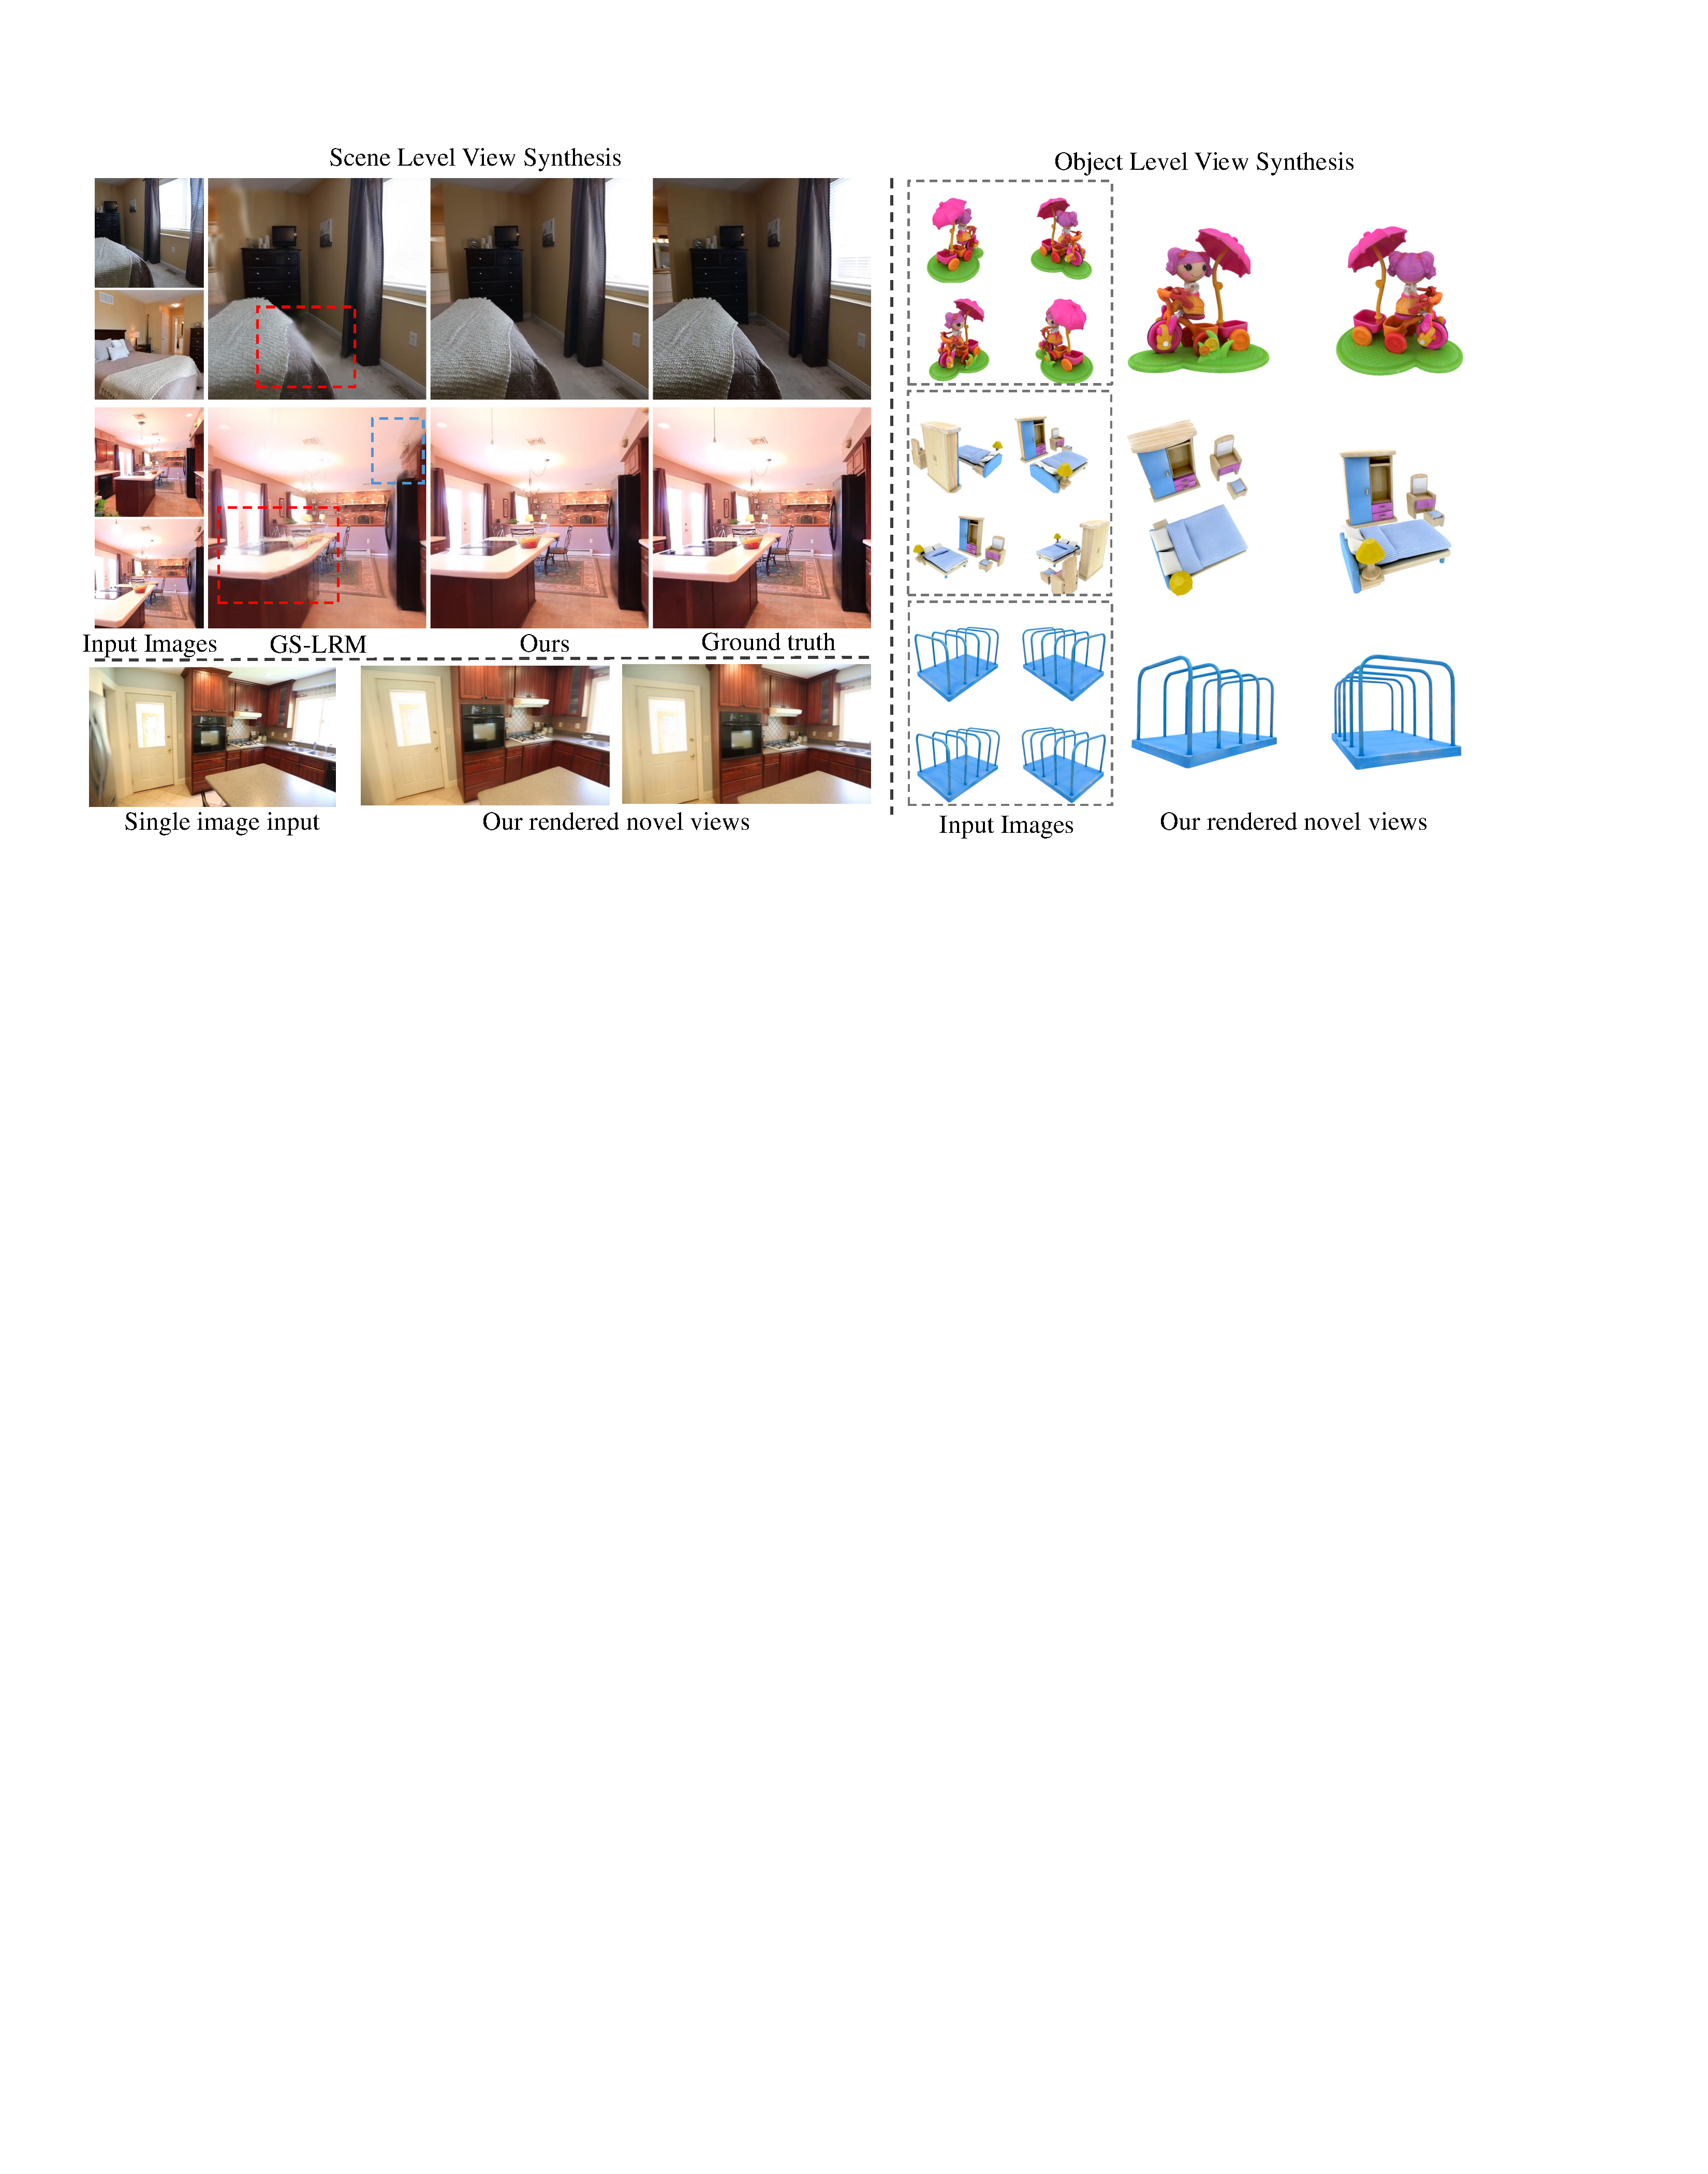
\includegraphics[width=0.99\textwidth]{figures/teaser.pdf}
    \vspace{-0.15in}
    \caption{\small{
    \paperName supports feed-forward novel view synthesis from sparse posed image inputs (even from a single view) on both objects and scenes. \paperName achieves significant quality improvements compared with the previous SOTA method, i.e., GS-LRM~\citep{zhang2024gslrmlargereconstructionmodel}. (Please zoom in for more details.)
    }
    } 
    \label{fig:teaser}
    \vspace{-0.20in}
\end{figure}

In this work, we aim to \emph{minimize 3D inductive biases} and push the boundaries of novel view synthesis with a fully data-driven approach. While some prior works have attempted to reduce 3D inductive biases~\citep{sitzmann2021lightfieldnetwork,sajjadi2022srt, kulhanek2022viewformer}, they still face challenges in scalability and achieving high rendering quality. We propose the \textbf{Large View Synthesis Model (LVSM)}, a novel transformer-based framework that synthesizes novel-view images from posed sparse-view inputs \emph{without predefined rendering equations or 3D structures, enabling accurate, training-efficient, and scalable novel view synthesis with photo-realistic quality} (as shown in Fig.~\ref{fig:teaser}).

To this end, we first introduce an \textbf{encoder-decoder LVSM}, removing handcrafted 3D representations and their rendering equations.
We use an encoder transformer to map the input (patchified) multi-view image tokens into a fixed number of 1D latent tokens, independent of the number of input views. These latent tokens are then processed by a decoder transformer, which uses target-view Plücker rays as positional embeddings to generate the target view’s image tokens, ultimately regressing the output pixel colors from a final linear layer. The encoder-decoder LVSM jointly learns a reconstructor (encoder), a scene representation (latent tokens), and a renderer (decoder) directly from data. By removing the need for predefined inductive biases in rendering and representation, \paperName offers improved generalization and achieves higher quality compared to NeRF- and GS-based approaches. 

Nevertheless, the encoder-decoder LVSM retains a key inductive bias: the use of an intermediate, albeit fully learned, scene representation. To further push the boundary, we propose a \textbf{decoder-only LVSM}, which adopts a single-stream transformer to directly convert input view tokens and target pose tokens into target view tokens, bypassing any intermediate representations. The decoder-only LVSM integrates novel view synthesis process into a holistic data-driven framework, achieving simultaneous scene reconstruction and rendering in a fully implicit manner with minimal 3D inductive bias.


We present a comprehensive evaluation of variants of both LVSM architectures. 
Notably, our models, trained on 2 or 4 input views, demonstrate strong zero-shot generalization to an unseen number of views, ranging from a single input to more than 10. Thanks to minimal inductive biases, our decoder-only model consistently outperforms the encoder-decoder variant in terms of quality, scalability, and zero-shot capability with varying numbers of input views. 
On the other hand, the encoder-decoder model achieves much faster inference speed due to its use of a fixed-length latent scene representation. Both models, benefiting from reduced 3D inductive biases, outperform previous methods, achieving state-of-the-art novel view synthesis quality across multiple object-level and scene-level benchmark datasets. Specifically, \textbf{our decoder-only LVSM surpasses previous state-of-the-art methods, such as GS-LRM, by a substantial margin of 1.5 to 3.5 dB PSNR}.  Our final models were trained on 64 A100 GPUs for 3-7 days, depending on the data type and model architecture, but we found that even with just 1--2 A100 GPUs for training, our model (with a decreased model and batch size) still outperforms all previous methods trained with equal or even more compute resources.


